Throughout the work reported on in this thesis, several designs of photodiode circuit were used to make sufficiently low noise measurements of photocurrents. For many of the experiments, it was necessary to measure a photocurrent's DC component, noise spectral density, and the size of calibration modulations in the photocurrent. Thus, the frequency response and noise characteristics of the photodiode circuits needed to be known.
\section{A Transimpedance Amplifier for Measuring the Dark Noise of Photodiodes}
\label{sec:appendix_dark_noise_tia}
A circuit which allowed for the reverse bias to be set and for the easy exchange of photodiodes was constructed. The photodiodes were connected to the circuit using pin header style connectors. To measure small amounts of current noise, a transimpedance amplifier with a large gain is needed. As the dark current for these photodiodes was expected to be of the order of 1\,\si{\micro\ampere}, the gain of the transimpedance amplifier was chosen to be $1\times10^6$ so that signals of the order 1\,V would be produced, and so a 1\,\si{\mega\ohm} resistor was used in the feedback path.
\par
The input noise of an op~amp depends on its input current noise, input voltage noise and the Johnson-Nyquist noise of the feedback resistor (e.g.~\cite[Figure~8.58]{Horowitz_and_Hill}). In this application, as the current noise that is to be measured is small and the feedback resistor is large, a TL071, a JFET style op~amp with low input current noise, was selected, and this selection of op~amp allowed the transimpedance amplifier to beat the noise requirement by a factor of several hundred (see Figure~\ref{fig:circuitappendixdarknoiseboxnoise}). As the photodiode has capacitance and the op~amp has finite bandwidth, a 2.2\,\si{\pico\farad} capacitor in parallel with the feedback resistor was needed to keep the circuit stable.
\par
Several methods of providing the reverse bias were tested. The first of these derived the reverse bias from a LM7815 regulator in combination with a variable resistor configured as a potential divider; this circuit is shown in Figure~\ref{fig:circuitappendixdarknoisetestbox1}. A similar circuit which was used in later experiments is shown in Figure~\ref{fig:circuitappendixdarknoisetestbox3}.
\begin{figure}
	\centering
	
\includegraphics[width=0.7\linewidth]{Circuit_appendix_dark_noise_test_box_1}
	\caption[A circuit used to measure the dark noise of photodiodes  under different reverse biases.]{The circuit used to measure the dark noise of photodiodes, represented by \textsc{Test\_PD}, under different reverse biases. The transimpedance amplifier has a 1\,\si{\mega\ohm} resistor (R2) in parallel with a 2.2\,\si{\pico\farad} capacitor (C2) in the feedback path of the TL071 op~amp. The reverse bias was generated by a potentiometer (R1) connected to an LM7815 voltage regulator. This voltage was low passed using C1. Note that the low pass corner frequency depends on the setting of R1.}
	\label{fig:circuitappendixdarknoisetestbox1}
\end{figure}
\begin{figure}
	\centering
	
\includegraphics[width=1\linewidth]{Circuit_appendix_dark_noise_test_box_2}
	\caption[A circuit used to measure the dark noise of photodiodes  under different reverse biases.]{The circuit used to measure the dark noise of photodiodes. The transimpedance amplifier used is identical to the one shown in Figure~\ref{fig:circuitappendixdarknoisetestbox1}. The reverse bias voltage was controlled with the potentiometer \textsc{BIAS\_ADJ}, and the reverse bias voltage was generated using an OP27 op~amp (OP27D) with a gain less than one.}
	\label{fig:circuitappendixdarknoisetestbox3}
\end{figure}
\par
To verify that this was a sufficiently quiet reverse bias voltage source that does not contaminate the measurements with noise, an ultra-quiet reverse bias reference was used to crosscheck a measurement; this circuit is shown in Figure~\ref{fig:circuitappendixdarknoisetestbox3}. By filtering the voltage made by a reference voltage \gls{ic} (AD587JNZ), this circuit provided a reverse bias with $5\,\si{\nano\volt/\sqrt{\hertz}}$ at 10\,Hz. The reverse bias of the FD10D was set to 1\,V in both circuits. In this circuit, the photodiode was soldered into it with minimal distance between the photodiode and the transimpedance amplifier. Figure~\ref{fig:pdchapterbiascrosscheck} shows that the regulator-potentiometer reverse bias voltage source is sufficiently quiet.
\begin{figure}
	\centering
	
\includegraphics[width=1\linewidth]{Circuit_appendix_dark_noise_test_box_3}
	\caption[Ultra-low bias voltage noise circuit used to validate measurements made with other circuits.]{The circuit used to check that reverse bias voltage noise was not contaminating dark noise measurements. To reach $5\,\si{\nano\volt/\sqrt{\hertz}}$ at 10\,Hz, a 10V low noise reference \gls{ic} (AD587JNZ) was used to generate the reverse bias. The output of this \gls{ic} was filtered by two low pass filters. The transimpedance amplifier used is identical to the one shown in Figure~\ref{fig:circuitappendixdarknoisetestbox1}}
	\label{fig:circuitappendixdarknoisetestbox2}
\end{figure}
\begin{figure}
	\centering
	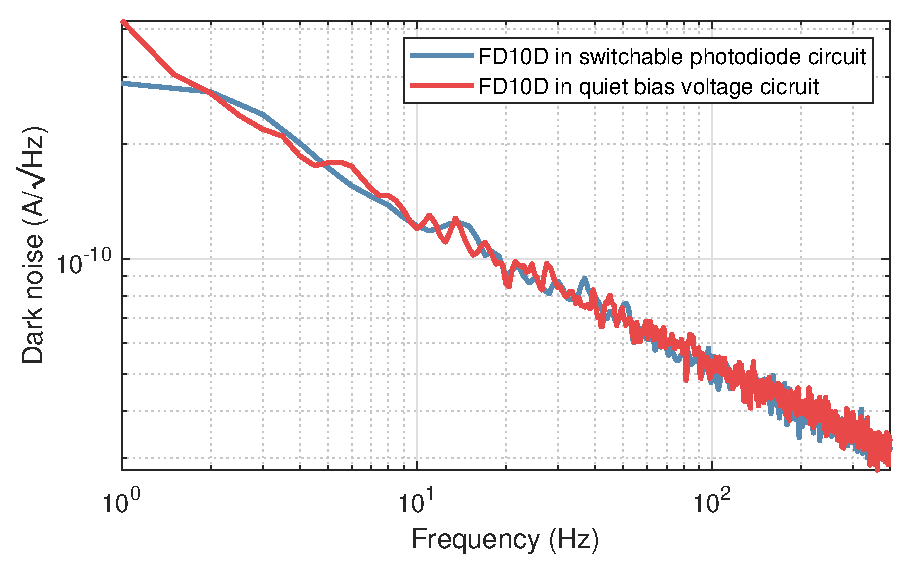
\includegraphics[width=1\linewidth]{Figures/PD_chapter_bias_cross_check}
	\caption[The FD10D shows the same dark noise in the ultra-low bias noise and regular test circuit.]{The FD10D was biased with 1\,V in the circuits shown in Figure~\ref{fig:circuitappendixdarknoisetestbox1} and Figure~\ref{fig:circuitappendixdarknoisetestbox2}. The low-noise fixed-bias circuit and the circuit with a settable-bias gave the same results, so we can be confident that the circuits shown in Figures \ref{fig:circuitappendixdarknoisetestbox1} and \ref{fig:circuitappendixdarknoisetestbox2} will produce measurements that are not contaminated by reverse bias noise or noise due to how the photodiode is connected to the circuit.}
	\label{fig:pdchapterbiascrosscheck}
\end{figure}
\clearpage
\subsection{Transfer Function}
The transfer function of the transimpedance amplifier shown in Figure~\ref{fig:circuitappendixdarknoisetestbox1} was measured under a variety of different physical constructions as this circuit's behaviour can be affected by stray capacitance. The measurements of these transfer functions are shown in Figure~\ref{fig:circuitappendixtransimpedanceamplifiertf}. When constructed from strip board and with the photodiode's anode and cathode cables near each other, there was of the order 10\,pF of stray capacitance, i.e.~it was as if the circuit had an extra 10\,pF capacitor between the inverting input of the op~amp and ground. By making this circuit on a prototyping board with less stray capacitance between the strips and by keeping the photodiode anode and cathode wires from forming a capacitor, the stray capacitance was reduced. The measurement matches the \textsc{\textsc{Liso}} (see Section~\ref{sec:circuit_appendix_liso}) simulation of this circuit. This was cross-checked using the \textsc{Matlab} function described in Section~\ref{sec:appendix_TIA_TF}.
\begin{figure}
	\centering
	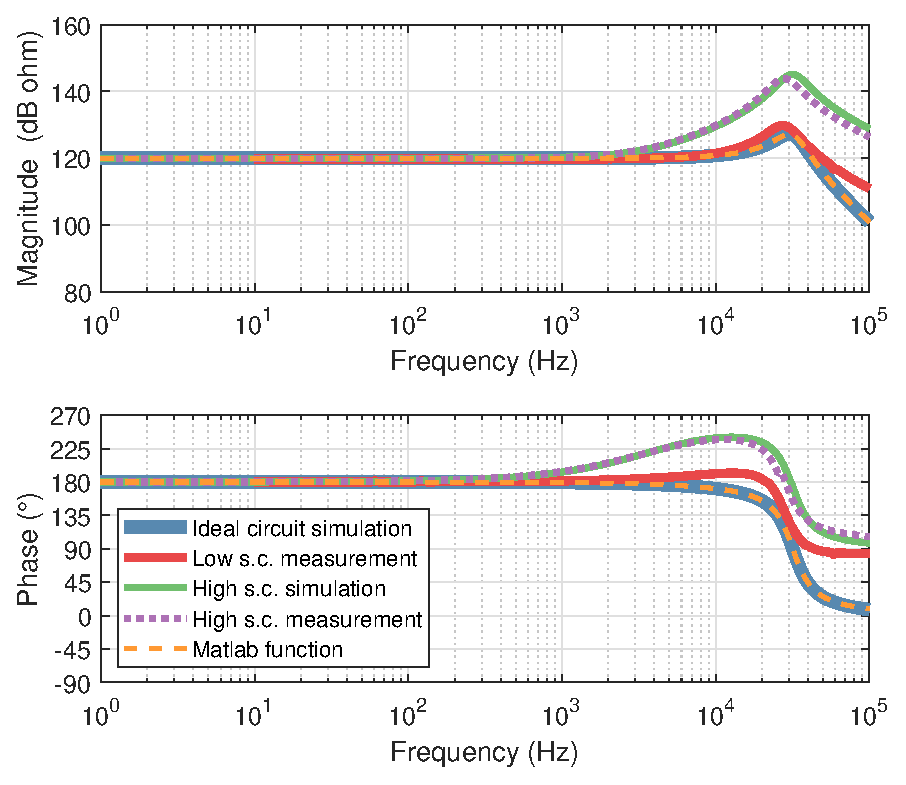
\includegraphics[width=1\linewidth]{Figures/Circuit_appendix_transimpedance_amplifier_TF}
	\caption[Transfer function of the transimpedance amplifier for measuring the dark noise of photodiodes.]{The transfer function between a current into the inverting input of the transimpedance amplifier design shown in Figure~\ref{fig:circuitappendixdarknoisetestbox1}, Figure~\ref{fig:circuitappendixdarknoisetestbox3} and Figure~\ref{fig:circuitappendixdarknoisetestbox2} was measured and simulated using \textsc{Liso}. A \textsc{Matlab} function (see Section~\ref{sec:appendix_TIA_TF}) was used to check the measurement and the simulation. This circuit is sensitive to stray capacitance (s.c.) at the inverting input of the TL071. The stray capacitance was reduced by changing the physical layout of the circuit.}
	\label{fig:circuitappendixtransimpedanceamplifiertf}
\end{figure}
\subsection{Noise Measurement}
The dark noise of the circuits described in Section~\ref{sec:appendix_dark_noise_tia} is shown in Figure~\ref{fig:circuitappendixdarknoiseboxnoise}. The shot noise of a typical photocurrent in a gravitational wave detector is several hundred times larger than the noise of this circuit. To measure the noise of the transimpedance amplifier, instead of a photodiode, a 470\,pF capacitor was connected between the inverting input of the op~amp and ground.
\begin{figure}
	\centering
	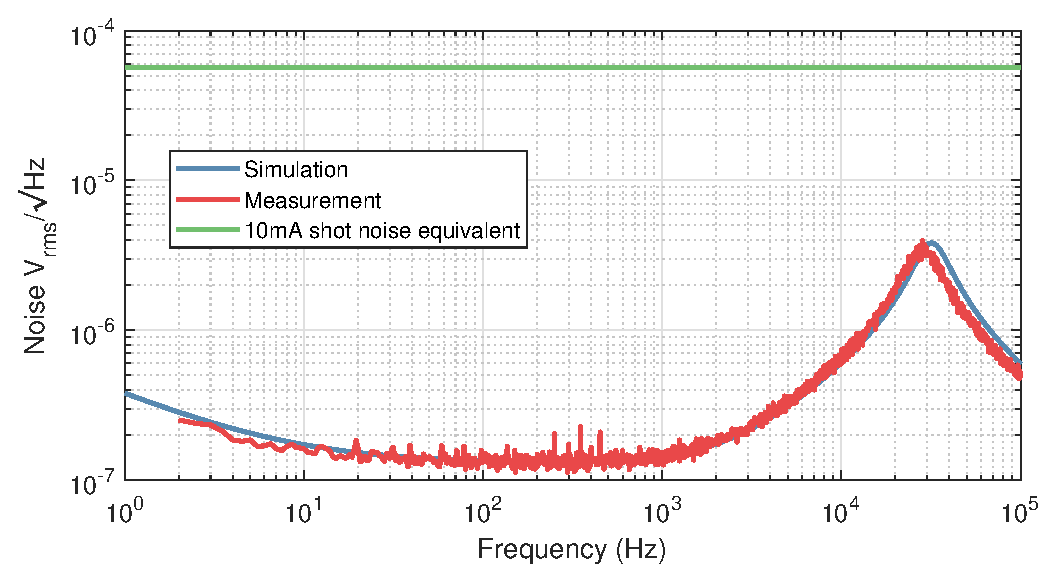
\includegraphics[width=1\linewidth]{Figures/Circuit_appendix_dark_noise_box_noise}
	\caption[Noise of the transimpedance amplifier for measuring the dark noise of photodiodes.]{At low frequencies, the noise of the transimpedance amplifier shown in Figure~\ref{fig:circuitappendixdarknoisetestbox1}, Figure~\ref{fig:circuitappendixdarknoisetestbox3} and Figure~\ref{fig:circuitappendixdarknoisetestbox2} is dominated by the low frequency voltage noise of the TL071. Above 10\,Hz, the noise of the circuit is dominated by the Johnson-Nyquist noise of the feedback resistor. At 30\,kHz, the impedance of the feedback network causes a noise peak. }
	\label{fig:circuitappendixdarknoiseboxnoise}
\end{figure}
\section{A Transimpedance Amplifier for Making Shot Noise limited Measurements of 10\,mA Photocurrents}
\label{sec:circuits_appendix_variable_bias_ad797}
A photodiode circuit with electronic noise $\sim\!25$ times lower than the shot noise of a 10\,mA current at frequencies between 100\,Hz to several MHz is shown in Figure~\ref{fig:pdchapterqetestcircuit}. Below 100\,Hz, the noise rises as $1/f$, and it equals the shot noise of a 10\,mA current at 0.1\,Hz. The noise for this circuit is shown in Figure~\ref{fig:pdchapterqetestcircuitnoise} and the transfer function is shown in Figure~\ref{fig:pdchapterqetestcircuittf}. While Figure~\ref{fig:pdchapterqetestcircuit} is specific to the experiment described in Section~\ref{sec:pd_chapter_reverse_bias_qe}, the design of the transimpedance part of this circuit (the AD797 and accompanying parts) was also used in Chapter \ref{chapter:in_air_MZ}. 
\par
The AD797~\cite{AD797} is a low-noise, high-speed op~amp. Without feedback, the AD797 has a higher output impedance than most common types of op~amp. As the AD797 is a fast device, the datasheet warns that consideration must be given to the interaction between the output impedance and a capacitive load to ground, including via the feedback network and the input network. As photodiodes have capacitance, care needs to be taken in designing transimpedance amplifiers that use AD797s. To avoid oscillations in similar circuits to the one shown in Figure~\ref{fig:pdchapterqetestcircuit}, the feedback capacitor may need a resistor in series with it (see \cite[p.14]{AD797}); however, in the circuit shown in Figure~\ref{fig:pdchapterqetestcircuit}, one was not required. Even so, if the photodiode is not biased or has a large area, this circuit may oscillate at a frequency between 10\,MHz--100\,MHz due to the capacitance of the photodiode. Every time a version of this circuit was made, an oscilloscope was used to check for such oscillations, as \textsc{Liso} does not model this behaviour. 
\par	
For convenience, the circuit shown in Figure~\ref{fig:pdchapterqetestcircuit} allowed for the reverse bias to be externally set. A DC reverse bias was created with a bench-top power supply, and low passed with a filter that had two poles at 16\,Hz. An AC component could be added onto the reverse bias with an op~amp configured to sum two input voltages.
\begin{figure}
	\centering
	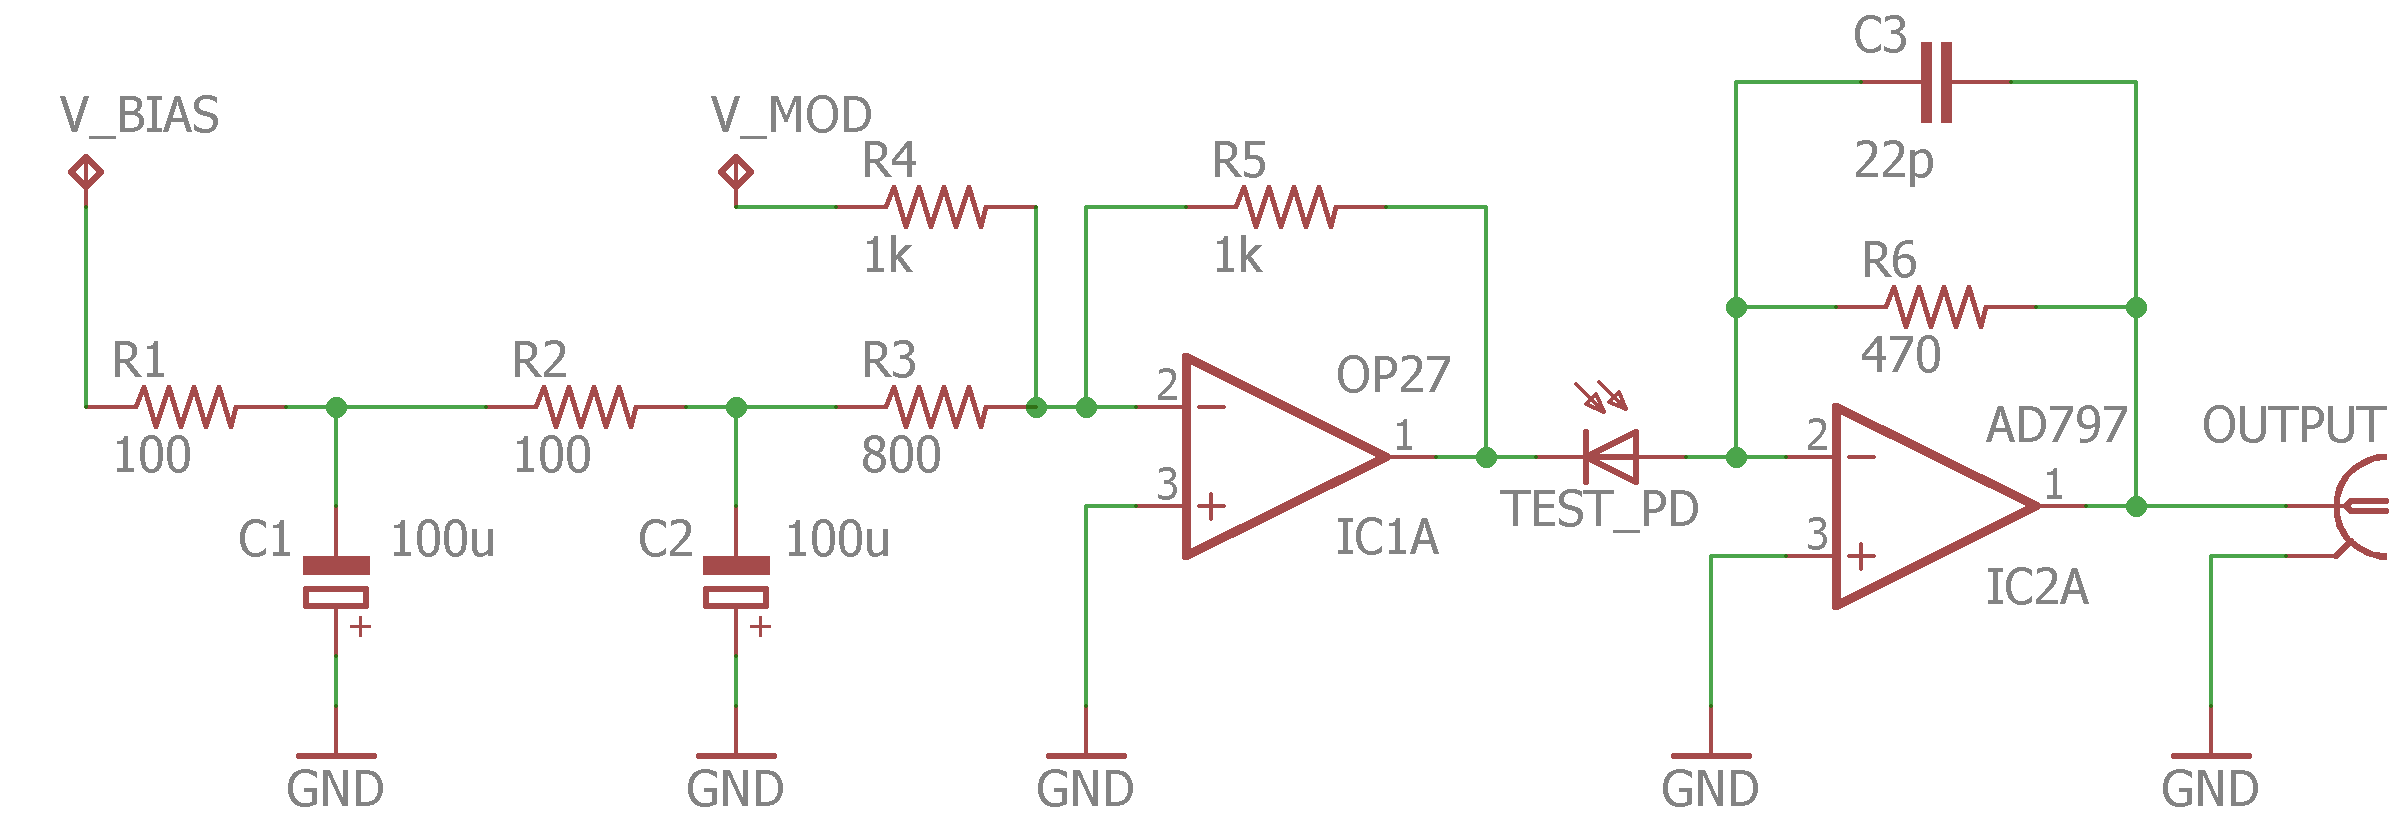
\includegraphics[width=1\linewidth]{Figures/PD_chapter_qe_test_circuit}
	\caption[Transimpedance amplifier designed for making shot noise limited measurements of photocurrents.]{The AD797 stage of the circuit (right) is a transimpedance amplifier for measuring the shot noise of 10\,mA photocurrents. The left-hand stage of the circuit is used to provide the reverse bias for the photodiode. One input of this stage is a low-pass filter with two poles at 16\,Hz. A bench-top power supply would be connected to this input (V\_BIAS). The other input, (V\_MOD), was used to provide a modulation to the reverse bias voltage.}
	\label{fig:pdchapterqetestcircuit}
\end{figure}
\begin{figure}
	\centering
	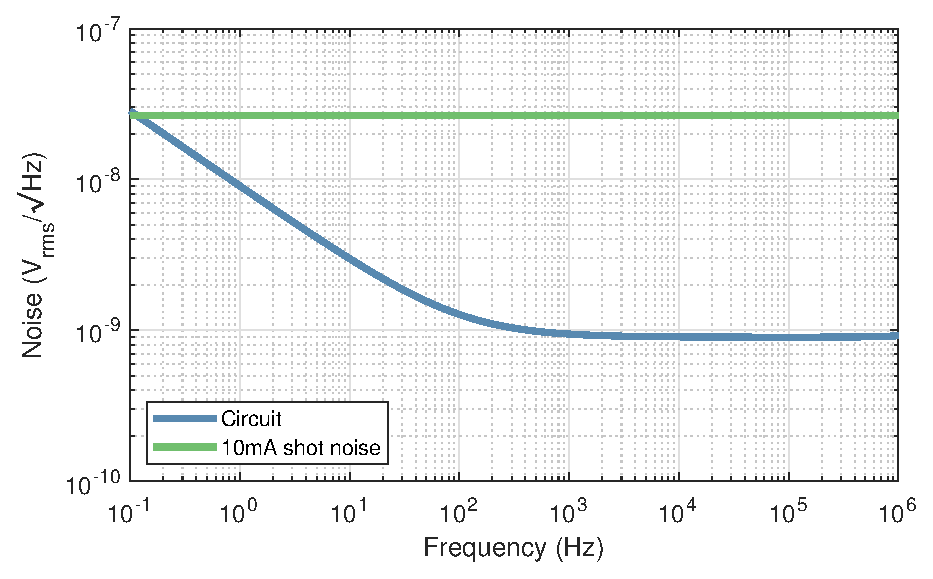
\includegraphics[width=1\linewidth]{Figures/PD_chapter_qe_test_circuit_noise}
	\caption[Transfer function of the transimpedance amplifier designed for making shot noise limited measurements of photocurrents.]{\textsc{Liso} simulation of the noise of the circuit used for measuring photocurrents of $\sim10\,\si{\milli\ampere}$. This circuit is shown in Figure~\ref{fig:pdchapterqetestcircuit}. Note that the simulation may not be accurate above 1\,MHz due to the unusually high output impedance of the AD797 and the capacitive load to ground. }
	\label{fig:pdchapterqetestcircuitnoise}
\end{figure}
\begin{figure}
	\centering
	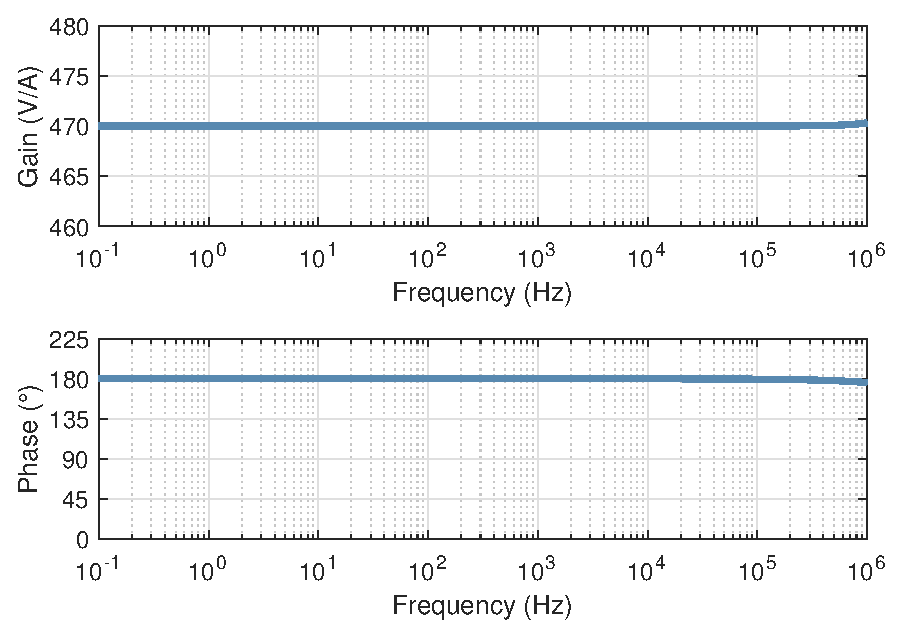
\includegraphics[width=1\linewidth]{Figures/PD_chapter_qe_test_circuit_TF}
	\caption[Noise of the transimpedance amplifier designed for making shot noise limited measurements of photocurrents.]{\textsc{Liso} simulation of the transfer function of the circuit used for measuring photocurrents of $\sim10\,\si{\milli\ampere}$. This circuit is shown in Figure~\ref{fig:pdchapterqetestcircuit}. Note that the simulation may not be accurate above 1\,MHz due to the unusually high output impedance of the AD797 and the capacitive load to ground.}
	\label{fig:pdchapterqetestcircuittf}
\end{figure}
\section{Simulations with \textsc{Liso}}
\label{sec:circuit_appendix_liso}
The behaviour of circuits was simulated using \textsc{Liso}. This software performs a nodal analysis to calculate the voltages at each point within a circuit. \textsc{Liso} can calculate the noise and transfer function of circuits that include op~amps. \textsc{Liso} has a variety of op~amps in its op~amp library and this can be easily expanded by specifying the noise properties, open loop gain and gain-bandwidth frequency of a new op~amp.
\section{Transfer Function Calculation With \textsc{Matlab}}
\label{sec:appendix_TIA_TF}
The open loop transfer function of an op~amp may be written as
\begin{equation}
A(s) = \frac{A_0}{\frac{A_0}{2\pi f_{\rm{GWB}}}s +1},
\end{equation}
where $A_0$ is the open-loop gain of the op~amp, $f_{\rm{GWB}}$ is the gain-bandwidth product of the op~amp and $s$ is the complex angular frequency. The transfer function between the input current and output voltage of a transimpedance amplifier is
\begin{equation}
H(s) = Z_{\rm{FB}}\frac{A(s)}{1+A(s)B(s)},
\label{eq:app_circuits_TIA_TF}
\end{equation}
where $B(s)$ is the transfer function of the components between the output pin of the op~amp and the inverting input of the op~amp, i.e.~the components in the feedback network of the transimpedance amplifier. $Z_{\rm{FB}}$ is the impedance seen by the current flowing from the output pin to the inverting input.
\par
Without a capacitor in parallel with the feedback resistor, $B(s) = \frac{1}{R_{\rm{FB}}C_{\rm{PD}}s+1}$. This can cause the circuit to be unstable because it can lead to the phase of the transfer function reaching or exceeding $180\si{\degree}$ as it crosses the unity gain point due to the photodiode's capacitance and the gain bandwidth product of the op~amp. To fix this problem, a capacitor should be added in parallel to the feedback resistor, and so 
\begin{equation}
B(s) = \frac{R_{\rm{FB}}C_{\rm{FB}}s + 1}{R_{\rm{FB}}(C_{\rm{FB}}+C_{\rm{PD}})s + 1}.
\end{equation}
The impedance seen by the current is 
\begin{equation}
Z_{\rm{FB}} = \frac{R_{\rm{FB}}}{R_{\rm{FB}}(C_{\rm{FB}}+C_{\rm{PD}})s + 1}.
\end{equation}
From Equation~(\ref{eq:app_circuits_TIA_TF}), $H(s)$ can be calculated with the following \textsc{Matlab} code:
\begin{lstlisting}
function [mag,phase] = photodiodeTransimpedance(cf, rf,cpd,gbw,A,w)
% cf = feedback capacitor (Farads). rf = feedback resistor (ohms)
% cpd = photodiode capacitance (Farads). 
% gbw = gain bandwidth of the op amp (Hz) 
% A = Open loop gain of the op amp. w = angular frequency range 
%that transfer function will be calculated over. 
A_s = tf(A,[A/(2*pi*gbw),1]);
B_s = tf([cf*rf,1],[rf*(cf+cpd),1]);
closedLoopAnalytic  = -tf(rf,[rf*(cf+cpd),1])*A_s/(1+A_s*B_s);
[mag,phase] = bode(closedLoopAnalytic,w);
mag = squeeze(mag);
phase = squeeze(phase);
end
\end{lstlisting}